% bei Standalone in documentclass noch:
% \RequirePackage{luatex85}

\documentclass[captions=tableheading, titlepage= firstiscover, parskip = half , bibliography=totoc]{scrartcl}
%paper = a5 für andere optinen
% titlepage= firstiscover
% bibliography=totoc für bibdateien
% parskip=half  Veränderung um Absätze zu verbessern

\usepackage{scrhack} % nach \documentclass
\usepackage[aux]{rerunfilecheck}
\usepackage{polyglossia}
\usepackage[style=numeric, backend=biber]{biblatex} % mit [style = alphabetic oder numeric] nach polyglossia
\addbibresource{lit.bib}
\setmainlanguage{german}

\usepackage[autostyle]{csquotes}
\usepackage{amsmath} % unverzichtbare Mathe-Befehle
\usepackage{amssymb} % viele Mathe-Symbole
\usepackage{mathtools} % Erweiterungen für amsmath
\usepackage{fontspec} % nach amssymb
% muss ins document: \usefonttheme{professionalfonts} % für Beamer Präsentationen
\usepackage{longtable}

\usepackage[
math-style=ISO,    % \
bold-style=ISO,    % |
sans-style=italic, % | ISO-Standard folgen
nabla=upright,     % |
partial=upright,   % /
]{unicode-math} % "Does exactly what it says on the tin."
\setmathfont{Latin Modern Math}
% \setmathfont{Tex Gyre Pagella Math} % alternativ

\usepackage[
% die folgenden 3 nur einschalten bei documenten
locale=DE,
separate-uncertainty=true, % Immer Fehler mit ±
per-mode=symbol-or-fraction, % m/s im Text, sonst \frac
]{siunitx}

% alternativ:
% per-mode=reciprocal, % m s^{-1}
% output-decimal-marker=., % . statt , für Dezimalzahlen

\usepackage[
version=4,
math-greek=default,
text-greek=default,
]{mhchem}

\usepackage[section, below]{placeins}
\usepackage{caption} % Captions schöner machen
\usepackage{graphicx}
\usepackage{grffile}
\usepackage{subcaption}

% \usepackage{showframe} Wenn man die Ramen sehen will

\usepackage{float}
\floatplacement{figure}{htbp}
\floatplacement{table}{htbp}

\usepackage{mhchem} %chemische Symbole Beispiel: \ce{^{227}_{90}Th+}


\usepackage{booktabs}

 \usepackage{microtype}
 \usepackage{xfrac}

 \usepackage{expl3}
 \usepackage{xparse}

 % \ExplSyntaxOn
 % \NewDocumentComman \I {}  %Befehl\I definieren, keine Argumente
 % {
 %    \symup{i}              %Ergebnis von \I
 % }
 % \ExplSyntaxOff

 \usepackage{pdflscape}
 \usepackage{mleftright}

 % Mit dem mathtools-Befehl \DeclarePairedDelimiter können Befehle erzeugen werden,
 % die Symbole um Ausdrücke setzen.
 % \DeclarePairedDelimiter{\abs}{\lvert}{\rvert}
 % \DeclarePairedDelimiter{\norm}{\lVert}{\rVert}
 % in Mathe:
 %\abs{x} \abs*{\frac{1}{x}}
 %\norm{\symbf{y}}

 % Für Physik IV und Quantenmechanik
 \DeclarePairedDelimiter{\bra}{\langle}{\rvert}
 \DeclarePairedDelimiter{\ket}{\lvert}{\rangle}
 % <name> <#arguments> <left> <right> <body>
 \DeclarePairedDelimiterX{\braket}[2]{\langle}{\rangle}{
 #1 \delimsize| #2
 }

\setlength{\delimitershortfall}{-1sp}

 \usepackage{tikz}
 \usepackage{tikz-feynman}

 \usepackage{csvsimple}
 % Tabellen mit \csvautobooktabular{"file"}
 % muss in table umgebung gesetzt werden


% \multicolumn{#Spalten}{Ausrichtung}{Inhalt}

\usepackage{hyperref}
\usepackage{bookmark}
\usepackage[shortcuts]{extdash} %nach hyperref, bookmark

\newcommand{\ua}[1]{_\symup{#1}}
\newcommand{\su}[1]{\symup{#1}}


\begin{document}

\section{Auswertung}

\subsection{Messung der Zeitkonstanten mit einer Entladekurve}

In dem ersten Teil des Versuches wird mit dem Oszilloskop die Entladekurve des
sich im RC-Kreis befindenden Kondensators betrachtet. Dem in Abbildung \ref{fig:thermodruck}
zu sehenden Thermodruck werden dabei 13 Wertepaare, bestehend aus der Zeit $t$
und der Kondensatorspannung $U\ua{C}$, entnommen und in den Graphen
(Abbildung \ref{fig:Messunga}) eingetragen. Mithilfe einer linearen Regression nach
Formel \eqref{eqn:FitMessungA} kann dann die Steigung ermittelt werden, deren
Kehrwert im Betrag der Zeitkonstante $RC$ entspricht.

\begin{align}
  \label{eqn:FitMessungA}
  ln \left( U\ua{C} \right) &= m \cdot t + b \\
  m    &= -\frac{1}{RC}
\end{align}

\begin{table}
  \centering
  \caption{Entnommene Wertepaare für die Spannungsamplituden zu verschiedenen
          Zeitpunkten des Entladevorgangs}
  \label{tab:MessungA}
  \begin{tabular}{c c || c c}
    \toprule $t \,\, in \,\, \su{ms}$ & $U\ua{C} \,\, in \,\, \su{V}$ &
             $t \,\, in \,\, \su{ms}$ & $U\ua{C} \,\, in \,\, \su{V}$ \\
    \midrule
    0.00 & 12.4 & 1.75 & 3.4 \\
    0.25 & 10   & 2.00 & 2.8 \\
    0.50 &  8.2 & 2.25 & 2.4 \\
    0.75 &  6.6 & 2.50 & 2   \\
    1.00 &  5.8 & 2.75 & 1.8 \\
    1.25 &  4.6 & 3.00 & 1.6 \\
    1.50 &  4   & -    & -   \\
    \bottomrule
  \end{tabular}
\end{table}

Mithilfe der linearen Regression ergibt sich dabei für die Zeitkonstante $RC$ ein
Wert von $RC = (0.00146 \pm 0.00003) \, \su{s}$.

\begin{figure}
  \centering
  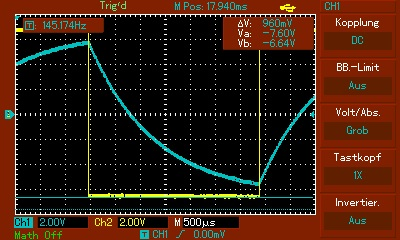
\includegraphics[width = 12 cm]{Sternchen.jpg}
  \caption{Thermodruck der in Messung x.1 betrachteten Entladekurve }
  \label{fig:thermodruck}
\end{figure}

\begin{figure}
  \centering
  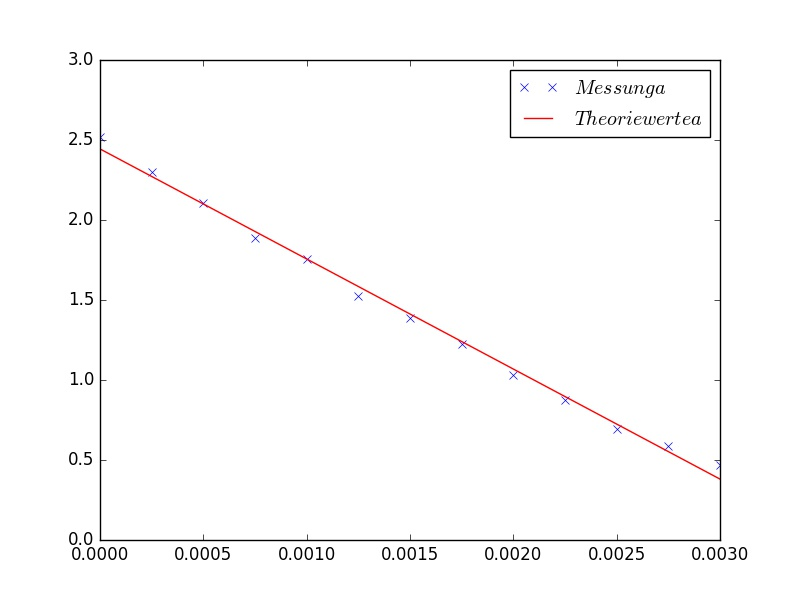
\includegraphics[width = 12 cm]{Messunga.jpg}
  \caption{gemessene Werte für $U\ua{C}$ aufgetragen gegen die Zeit $t$}
  \label{fig:Messunga}
\end{figure}

%Eingügen der Grafik mit den eingetragenenen Werten

\newpage

\subsection{Bestimmung der Zeitkonstanten über Messung der zeitabhängigen Spannungsamplitude}

In der zweiten Messung des Versuches wurde mithilfe des Oszilloskopes die
Spannungsamplitude an dem Kondensator in Abhängigkeit der Frequenz gemessen,
da auch diese eine Abhängigkeit von der Zeitkonstante aufweist.
Das Verhältnis von gemessener Amplitude $U\ua{C}$ und der anliegenden
Ausgangsspannung wird $U\ua{G}$ logarythmisch in dem Graphen aufgetragen und
mithilfe einer Regressionskurve nach Formel \eqref{eqn:FitMessungB} kann dann
die Zeitkonstante RC bestimmt werden, die in Formel \eqref{eqn:FitMessungB} der
Konstante a entspricht.

\begin{equation}
  A(\nu) = \frac{U\ua{G}}{ \sqrt{ 1 + ( 2 \cdot \pi \cdot \nu )^2 \cdot a^2}}
  \label{eqn:FitMessungB}
\end{equation}

Aus der Abbildung \ref{fig:Messungb} ergibt sich somit mit der Regressionskurve
für die Zeitkonstante folgender Wert:

\begin{equation}
  RC = a = (0.00130 \pm 0.00002) \, \su{s} .
\end{equation}

\begin{figure}
  \centering
  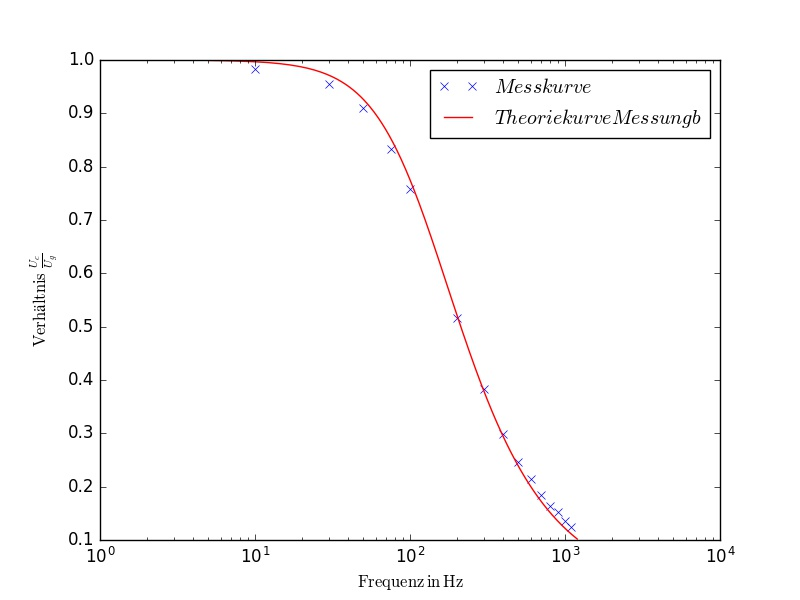
\includegraphics[width = 12 cm]{Messungb.jpg}
  \caption{Verhältnis der gemessenen Spannungsamplituden $U\ua{C}$ und der
           Ausgangsspannung $U\ua{0}$ aus Tabelle \ref{tab:MessungB} aufgetragen
          gegen die Frequenz $\nu$}
  \label{fig:Messungb}
\end{figure}

\begin{table}
  \centering
  \caption{Gemessene Spannungsamplituden der Kondensatorspannung für verschiedene
           angelegte Frequenzen $\nu$}
  \label{tab:MessungB}
  \begin{tabular}{ c c c || c c c }
    \toprule $\nu \,\, in \,\, \su{Hz}$ & $U\ua{C} \,\, in \,\, \su{V}$ & $U\ua{C} \,\, in \,\, \su{V}$ &
             $\nu \,\, in \,\, \su{Hz}$ & $U\ua{C} \,\, in \,\, \su{V}$ & $U\ua{C} \,\, in \,\, \su{V}$ \\
    \midrule
     10 & 14.1  & 14.35 &  500 & 3.48 & 14.1 \\
     30 & 13.62 & 14.25 &  600 & 3.01 & 14.1 \\
     50 & 12.91 & 14.20 &  700 & 2.61 & 14.1 \\
     75 & 11.88 & 14.25 &  800 & 2.30 & 14.1 \\
    100 & 10.77 & 14.2  &  900 & 2.14 & 14.1 \\
    200 &  7.29 & 14.13 & 1000 & 1.90 & 14.0 \\
    300 &  5.39 & 14.1  & 1100 & 1.74 & 13.9 \\
    400 &  4.20 & 14.1  & -    & -    & -    \\
    \bottomrule
  \end{tabular}
\end{table}

\subsection{Messung der Zeitkonstante über die Phasenverschiebung}

In dem dritten Teil des Experimentes wird die Zeitkonstante noch einmal über
den Phasenverschub bestimmt, der wie in Formel ?? zu sehen ist sowohl
von der Frequenz als auch von der Zeitkonstante abhängig ist. Die gemessenen Werte
für die zeitliche Verzögerung $a$ sowie die Schwingungsdauer $b$ und die daraus
resultierende Phasenverschiebung $\varphi$ sind in der folgenden Tabelle zu sehen.

\begin{table}
  \centering
  \caption{Gemessene Werte für die Parameter a und b sowie die resultierende Phasenverschiebung}
  \label{tab:Phasenverschiebung}
  \begin{tabular}{c c c c}
    \toprule $\nu \,\, in  \,\, \su{Hz}$ & $a \,\, in \,\, \su{ms}$ &
             $b \,\, in \,\, \su{ms}$ & $\varphi \,\, in \,\, \su{rad}$ \\
    \midrule
     10 & 99.2 & 100.1 & 0.055 \\
     30 & 32.0 &  33.3 & 0.253 \\
     50 & 18.4 &  20.0 & 0.506 \\
     75 & 12.0 &  13.3 & 0.631 \\
    100 & 8.80 &  10.0 & 0.754 \\
    200 & 4.20 &  5.00 & 1.005 \\
    300 & 2.68 &  3.33 & 1.226 \\
    400 & 2.00 &  2.50 & 1.257 \\
    500 & 1.60 &  2.00 & 1.257 \\
    600 & 1.32 &  1.67 & 1.317 \\
    700 & 1.12 &  1.43 & 1.362 \\
    800 & 1.00 &  1.25 & 1.257 \\
    900 & 0.88 &  1.11 & 1.302 \\
    1000 & 0.76 &  1.00 & 1.508 \\
    1100 & 0.66 &  0.91 & 1.726 \\
    \bottomrule
  \end{tabular}
\end{table}

Die gemessene Phasenverschiebung wird in Abbildung ?? gegen die eingestellte
Frequenz aufgetragen. Über eine Regressionskurve nach Formel \eqref{eqn:regressionC},
in der der Parameter a der zu bestimmenden Zeitkonstante RC entspricht.

\begin{equation}
  \varphi = \arctan (- 2 \pi \nu a)
  \label{eqn:regressionC}
\end{equation}

Für RC ergibt sich somit der folgende Wert:

\begin{equation}
  RC = (0.00139 \pm 0.00013) \, \su{s} .
\end{equation}




















\end{document}
